%In the name of Allah(Gad)
\documentclass[12pt]{article}
\setlength{\headheight}{15pt}

\usepackage{graphicx}
\usepackage{fancyhdr}
\usepackage{hyperref}


\title{
    \textbf{\Huge In the name of Allah}\\
    \vspace{2in}
    \textbf{Computer Workshop}\\
    Final Assignment\\
    Integration of Tools and Practices\\
    \vspace{0.1in}
    \large Iran University of Science and Technology\\
    \large Department of Computer Engin
    \vspace{0.5in}
}


\author{
    \vspace{0.1in}
    Seyyed Mahdi Mousavi\\
    Computer Workshop 02-03\\
    \vspace{0.2in}
}
\date{5 bahman, 1402}


\begin{document}
\pagestyle{fancy}

\maketitle
\tableofcontents
\newpage

\maketitle

\section{Git and GitHub}
\subsection{Repository Initialization and Commits}
\begin{enumerate}
    \item Opening the GitHub website
    \item Click the "New" button on the top left.
    \item Enter the name of your desired repository in the "Repository name" section.
    \item Insert a brief explanation about the repository in the "Description" section.
    \item Click "Create repository".
    \item Now, in the system, within the desired folder, enter the command "git init".
    \item Then enter the command "git remot add <url>" (replace "url" with the url from the "Code" page of the repository).
\end{enumerate}

\subsection{GitHub Actions for LaTeX Compilation}
\begin{enumerate}
    \item Creating main.yml file
    \item Placing main.yml file inside the .github/workflows folder
    \item Adding the ".github" folder
    \item Committing changes
    \item Pushing
    \item With main.yml configured correctly, actions should automatically execute once the latest Commit is tagged with a v*.*.* number. Finally, the code is pushed to GitHub with the command "git push origin v*.*.*".
\end{enumerate}

\section{Exploration Tasks}
\subsection{Vim Advanced Features}
\begin{enumerate}
    \item \textbf{Macro recording:} Macro recording allows you to record a series of commands and then repeat them later whenever needed.
        \begin{enumerate}
            \item Enter record mode by pressing Ctrl+R
            \item Perform the desired tasks that you want to record
            \item When the recording is done, press Ctrl+R again to stop recording.
            \item Press Ctrl+R to play the macro again.
        \end{enumerate}

    \item \textbf{Multiple Registers:} Vim uses multiple "registers" that allow you to quickly store and retrieve text. These registers can be used to store long lists or complex text formats such 
        \begin{enumerate}
            \item Enter the register command and type a letter to create a new register:\\
            :register 'letter'
            \item Enter the content you want to store by typing it on the command line.
            \item Repeat this process as many times as needed to create multiple registers.
            \item Retrieve the text from the register whenever you need it.
        \end{enumerate}

    \item \textbf{Plugins:} Vim is extremely customizable through plugins. There are numerous plugins available that extend the core capabilities of Vim.
\end{enumerate}

\subsection{Memory profiling}
    \subsubsection{Memory Leak:}
        Memory leaks in C are usually caused by dynamically allocated memory that is never released back to the system. Over time, this unused memory leads to a build-up of unreclaimed memory which eventually consumes all available memory. This can cause program crashes or system instability, making it a serious performance issue.
    \subsubsection{Memory profilers:}
        Valgrind is a software testing and debugging tool for C/C++ programs. It can be used to optimize memory usage, detect memory leaks, find memory corruption/access issues, and help with code profile and performance analysis in C/C++ programs. It is a powerful tool for detecting memory issues and improving code efficiency.

\subsection{GNU/Linux Bash Scripting}
\subsubsection{fzf}
    \begin{itemize}
        \item \textbf{Fuzzy searching}, is a type of search algorithm that matches items in a database or list with similar properties, instead of exact matches. It is useful for cases where items may have minor spelling mistakes or alternative spellings, and for searches that require a broader definition of a term or concept. 
        \item \texttt{ls | fzf:} This command uses the "ls" command to list all the files in the current directory and then passes the output as an argument to the "fzf" command. The "fzf" command performs fuzzy searching on the output of the "ls" command, and then displays the results on the terminal.
    \end{itemize}
\subsubsection{Using fzf to find your favorite PDF}
Here's the command you need to write to list all the pdfs in the current directory and use fzf to select one.\\
\Large \texttt{fd pdf | fzf}
\begin{figure}
    \centering
    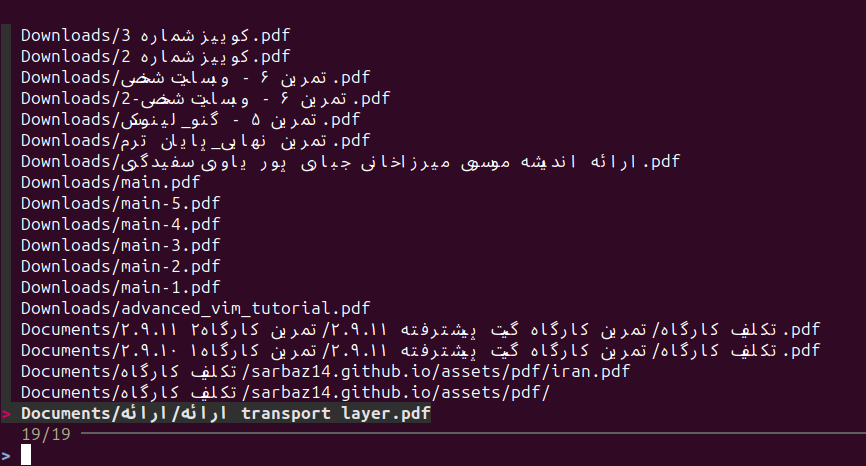
\includegraphics[width=1\textwidth]{fzf.png}
    \caption{\texttt{fd pdf | fzf}}
\end{figure}

\subsubsection{Opening the file using Zathura}
We use the command below to open the PDF that was generated by the commands earlier.\\
\Large \texttt{zathura \$(fd pdf | fzf)}
\begin{figure}
    \centering
    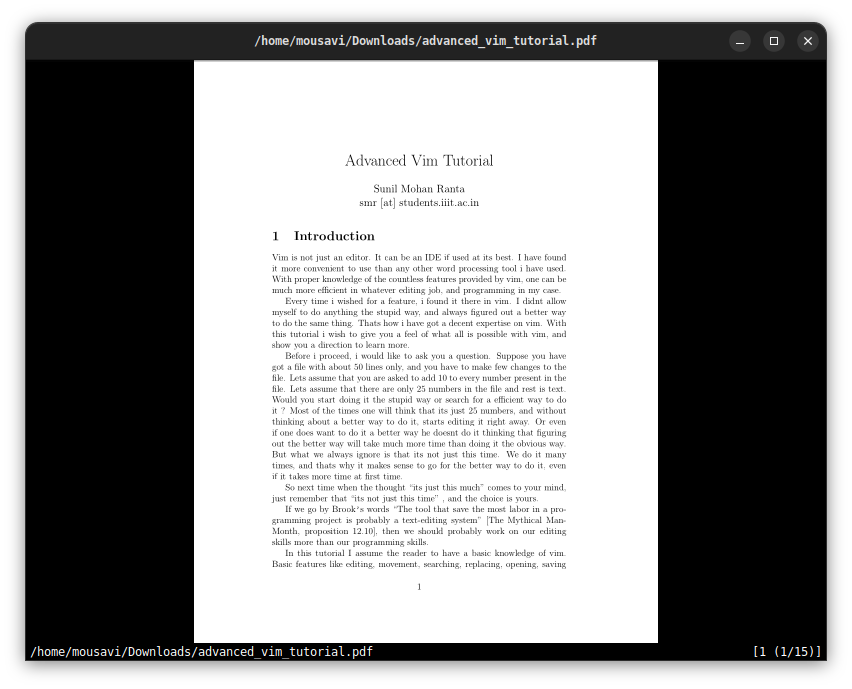
\includegraphics[width=0.75\textwidth]{zathura.png}
    \caption{\texttt{zathura \$(fd pdf | fzf)}}
\end{figure}

\section{Git and FOSS}
\subsection{README.md}
You can view the "README" file in \href{https://github.com/sarbaz14/latex/blob/master/README.md}{this} link

\subsection{Issues}
\begin{figure}[!h]
    \centering
    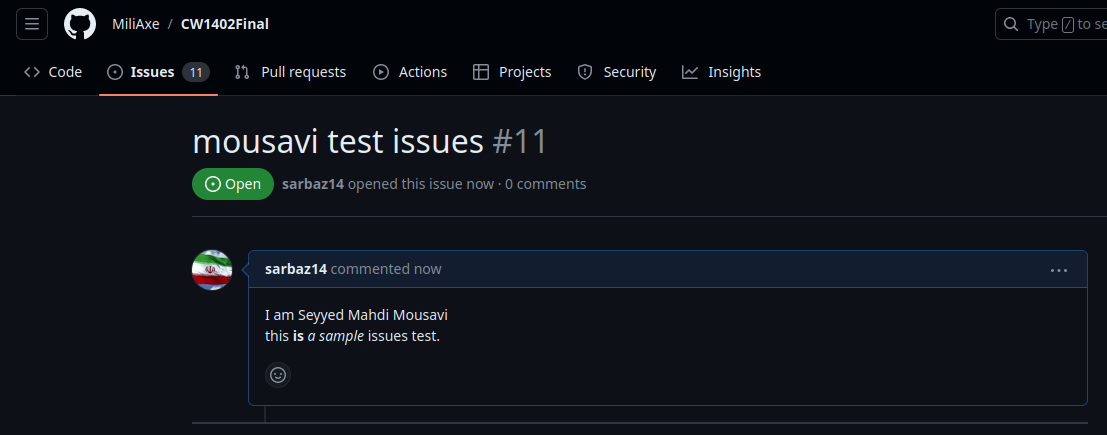
\includegraphics[width=1\textwidth]{issues.png}
    \caption{this is my issues}
\end{figure}

\end{document}

